%==============================================================================
% tento soubor pouzijte jako zaklad
% this file should be used as a base for the thesis
% Autoři / Authors: 2008 Michal Bidlo, 2016 Jaroslav Dytrych
% Kontakt pro dotazy a připomínky: dytrych@fit.vutbr.cz
% Contact for questions and comments: dytrych@fit.vutbr.cz
%==============================================================================
% kodovani: UTF-8 (zmena prikazem iconv, recode nebo cstocs)
% encoding: UTF-8 (you can change it by command iconv, recode or cstocs)
%------------------------------------------------------------------------------
% zpracování / processing: make, make pdf, make clean
%==============================================================================
% Soubory, které je nutné upravit: / Files which have to be edited:
%   xchrip00_sep-20-literatura-bibliography.bib - literatura / bibliography
%   xchrip00_sep-01-kapitoly-chapters.tex - obsah práce / the thesis content
%   xchrip00_sep-30-prilohy-appendices.tex - přílohy / appendices
%==============================================================================
\documentclass[slovak,zadani]{fitthesis} % bez zadání - pro začátek práce, aby nebyl problém s překladem
%\documentclass[english]{fitthesis} % without assignment - for the work start to avoid compilation problem
%\documentclass[zadani]{fitthesis} % odevzdani do wisu - odkazy jsou barevné
%\documentclass[english,zadani]{fitthesis} % for submission to the IS FIT - links are color
%\documentclass[zadani,print]{fitthesis} % pro tisk - odkazy jsou černé
%\documentclass[zadani,cprint]{fitthesis} % pro barevný tisk - odkazy jsou černé, znak VUT barevný
%\documentclass[english,zadani,print]{fitthesis} % for the color print - links are black
%\documentclass[english,zadani,cprint]{fitthesis} % for the print - links are black, logo is color
% * Je-li práce psaná v anglickém jazyce, je zapotřebí u třídy použít 
%   parametr english následovně:
%   If thesis is written in english, it is necessary to use 
%   parameter english as follows:
%      \documentclass[english]{fitthesis}
% * Je-li práce psaná ve slovenském jazyce, je zapotřebí u třídy použít 
%   parametr slovak následovně:
%   If the work is written in the Slovak language, it is necessary 
%   to use parameter slovak as follows:
%      \documentclass[slovak]{fitthesis}
% * Je-li práce psaná v anglickém jazyce se slovenským abstraktem apod., 
%   je zapotřebí u třídy použít parametry english a enslovak následovně:
%   If the work is written in English with the Slovak abstract, etc., 
%   it is necessary to use parameters english and enslovak as follows:
%      \documentclass[english,enslovak]{fitthesis}

% Základní balíčky jsou dole v souboru šablony fitthesis.cls
% Basic packages are at the bottom of template file fitthesis.cls
% zde můžeme vložit vlastní balíčky / you can place own packages here

% Kompilace po částech (rychlejší, ale v náhledu nemusí být vše aktuální)
% Compilation piecewise (faster, but not all parts in preview will be up-to-date)
\usepackage{subfiles}

% Nastavení cesty k obrázkům
% Setting of a path to the pictures
\graphicspath{{obrazky/}{./obrazky/}}
%\graphicspath{{obrazky-figures/}{../obrazky-figures/}}

%---rm---------------
\renewcommand{\rmdefault}{lmr}%zavede Latin Modern Roman jako rm / set Latin Modern Roman as rm
%---sf---------------
\renewcommand{\sfdefault}{qhv}%zavede TeX Gyre Heros jako sf
%---tt------------
\renewcommand{\ttdefault}{lmtt}% zavede Latin Modern tt jako tt

% vypne funkci šablony, která automaticky nahrazuje uvozovky,
% aby nebyly prováděny nevhodné náhrady v popisech API apod.
% disables function of the template which replaces quotation marks
% to avoid unnecessary replacements in the API descriptions etc.
\csdoublequotesoff

% =======================================================================
% balíček "hyperref" vytváří klikací odkazy v pdf, pokud tedy použijeme pdflatex
% problém je, že balíček hyperref musí být uveden jako poslední, takže nemůže
% být v šabloně
% "hyperref" package create clickable links in pdf if you are using pdflatex.
% Problem is that this package have to be introduced as the last one so it 
% can not be placed in the template file.
\ifWis
\ifx\pdfoutput\undefined % nejedeme pod pdflatexem / we are not using pdflatex
\else
  \usepackage{color}
  \usepackage[unicode,colorlinks,hyperindex,plainpages=false,pdftex]{hyperref}
  \definecolor{links}{rgb}{0.4,0.5,0}
  \definecolor{anchors}{rgb}{1,0,0}
  \def\AnchorColor{anchors}
  \def\LinkColor{links}
  \def\pdfBorderAttrs{/Border [0 0 0] }  % bez okrajů kolem odkazů / without margins around links
  \pdfcompresslevel=9
\fi
\else % pro tisk budou odkazy, na které se dá klikat, černé / for the print clickable links will be black
\ifx\pdfoutput\undefined % nejedeme pod pdflatexem / we are not using pdflatex
\else
  \usepackage{color}
  \usepackage[unicode,colorlinks,hyperindex,plainpages=false,pdftex,urlcolor=black,linkcolor=black,citecolor=black]{hyperref}
  \definecolor{links}{rgb}{0,0,0}
  \definecolor{anchors}{rgb}{0,0,0}
  \def\AnchorColor{anchors}
  \def\LinkColor{links}
  \def\pdfBorderAttrs{/Border [0 0 0] } % bez okrajů kolem odkazů / without margins around links
  \pdfcompresslevel=9
\fi
\fi
% Řešení problému, kdy klikací odkazy na obrázky vedou za obrázek
% This solves the problems with links which leads after the picture
\usepackage[all]{hypcap}

\usepackage[ruled]{algorithm2e}
\usepackage{tikz}
\usepackage{amsthm}
\usepackage{subcaption}
\newtheorem*{definition}{Definícia}
\def\checkmark{\tikz\fill[scale=0.4](0,.35) -- (.25,0) -- (1,.7) -- (.25,.15) -- cycle;} 

\makeatletter
\newcommand\footnoteref[1]{\protected@xdef\@thefnmark{\ref{#1}}\@footnotemark}
\makeatother

% Informace cls práci/projektu / Information about the thesis
%---------------------------------------------------------------------------
\projectinfo{
  %Prace / Thesis
  project={SP},            %typ práce BP/SP/DP/DR  / thesis type (SP = term project)
  year={2018},             % rok odevzdání / year of submission
  date=\today,             % datum odevzdání / submission date
  %Nazev prace / thesis title
  title.cs={Automatizované testování systému Fitcrack},  % název práce v češtině či slovenštině (dle zadání) / thesis title in czech language (according to assignment)
  title.en={Automated Testing of Fitcrack System}, % název práce v angličtině / thesis title in english
  %title.length={14.5cm}, % nastavení délky bloku s titulkem pro úpravu zalomení řádku (lze definovat zde nebo níže) / setting the length of a block with a thesis title for adjusting a line break (can be defined here or below)
  %Autor / Author
  author.name={Juraj},   % jméno autora / author name
  author.surname={Chripko},   % příjmení autora / author surname 
  %author.title.p={Bc.}, % titul před jménem (nepovinné) / title before the name (optional)
  %author.title.a={Ph.D.}, % titul za jménem (nepovinné) / title after the name (optional)
  %Ustav / Department
  department={UIFS}, % doplňte příslušnou zkratku dle ústavu na zadání: UPSY/UIFS/UITS/UPGM / fill in appropriate abbreviation of the department according to assignment: UPSY/UIFS/UITS/UPGM
  % Školitel / supervisor
  supervisor.name={Radek},   % jméno školitele / supervisor name 
  supervisor.surname={Hranický},   % příjmení školitele / supervisor surname
  supervisor.title.p={Ing.},   %titul před jménem (nepovinné) / title before the name (optional)
  supervisor.title.a={},    %titul za jménem (nepovinné) / title after the name (optional)
  % Klíčová slova / keywords
  keywords.cs={Fitcrack, BOINC, testovanie, jednotkové testy, integračné testy}, % klíčová slova v českém či slovenském jazyce / keywords in czech or slovak language
  keywords.en={Fitcrack, BOINC, testing, unit testing, integration testing}, % klíčová slova v anglickém jazyce / keywords in english
  % Abstrakt / Abstract
  abstract.cs={Táto práca si kladie za cieľ navrhnúť a implementovať automatizované testy pre systém Fitcrack, distribuovaný systém na lámanie hesiel.
Testy musia byť takisto distribuované a prenositeľné, keďže časť systému pracuje na klientských zariadeniach. 
Pre väčšie pokrytie testovacích prípadov sú použité viaceré techniky testovania. 
V práci je rozobraná teória fungovania systému Fitcrack, ako aj požiadavky na testy, teória prístupov k testovania a ich jednotlivý prínos pri odhaľovaní chýb.
Práca ďalej obsahuje návrh systémových testov s ohľadom na zistenia cls fungovaní systému Fitcrack.
\todo{Prečítať a prerobiť.}}, % abstrakt v českém či slovenském jazyce / abstract in czech or slovak language
  abstract.en={This thesis aims to design and implement automated tests for Fitcrack, distributed password cracking system. 
Tests also have to be distibuted and cross-platform, as part of the system operates on client's machine.
For better code coverage multiple testing technics are combined.
In thesis is discussed Fitcrack functioning theory as well as requirements for tests, software testing principles and their contribution to error detection.
Thesis further includes Fitcrack tests design with consideration for findings about Fitcrack.}, % abstrakt v anglickém jazyce / abstract in english
  % Prohlášení (u anglicky psané práce anglicky, u slovensky psané práce slovensky) / Declaration (for thesis in english should be in english)
  declaration={Prehlasujem, že som túto bakalárskou prácu vypracoval samostatne pod vedením pana Ing. Radka Hranického.
%Další informace mi poskytli...
Uvedl jsem všechny literární prameny a publikace, ze kterých jsem čerpal.},
  %declaration={Hereby I declare that this bachelor's thesis was prepared as an original author’s work under the supervision of Mr. X
% The supplementary information was provided by Mr. Y
% All the relevant information sources, which were used during preparation of this thesis, are properly cited and included in the list of references.},
  % Poděkování (nepovinné, nejlépe v jazyce práce) / Acknowledgement (optional, ideally in the language of the thesis)
  acknowledgment={Rád by som poďakoval vedúcemu práce Ing. Radkovi Hranickému za odbornú pomoc, usmerňovanie pri riešení práce a trpezlivosť.},
  %acknowledgment={Here it is possible to express thanks to the supervisor and to the people which provided professional help
%(external submitter, consultant, etc.).},
  % Rozšířený abstrakt (cca 3 normostrany) - lze definovat zde nebo níže / Extended abstract (approximately 3 standard pages) - can be defined here or below
  %extendedabstract={Do tohoto odstavce bude zapsán rozšířený výtah (abstrakt) práce v českém (slovenském) jazyce.},
  %faculty={FIT}, % FIT/FEKT/FSI/FA/FCH/FP/FAST/FAVU/USI/DEF
  faculty.cs={Fakulta informačních technologií}, % Fakulta v češtině - pro využití této položky výše zvolte fakultu DEF / Faculty in Czech - for use of this entry select DEF above
  faculty.en={Faculty of Information Technology}, % Fakulta v angličtině - pro využití této položky výše zvolte fakultu DEF / Faculty in English - for use of this entry select DEF above
  department.cs={Ústav informačních systémů}, % Ústav v češtině - pro využití této položky výše zvolte ústav DEF nebo jej zakomentujte / Department in Czech - for use of this entry select DEF above or comment it out
  department.en={Department of Information Systems} % Ústav v angličtině - pro využití této položky výše zvolte ústav DEF nebo jej zakomentujte / Department in English - for use of this entry select DEF above or comment it out
}

% Rozšířený abstrakt (cca 3 normostrany) - lze definovat zde nebo výše / Extended abstract (approximately 3 standard pages) - can be defined here or above
%\extendedabstract{Do tohoto odstavce bude zapsán výtah (abstrakt) práce v českém (slovenském) jazyce.}

% nastavení délky bloku s titulkem pro úpravu zalomení řádku - lze definovat zde nebo výše / setting the length of a block with a thesis title for adjusting a line break - can be defined here or above
%\titlelength{14.5cm}


% řeší první/poslední řádek odstavce na předchozí/následující stránce
% solves first/last row of the paragraph on the previous/next page
\clubpenalty=10000
\widowpenalty=10000

\begin{document}
  % Vysazeni titulnich stran / Typesetting of the title pages
  % ----------------------------------------------
  \maketitle
  % Obsah
  % ----------------------------------------------
  \setlength{\parskip}{0pt}

  {\hypersetup{hidelinks}\tableofcontents}
  
  % Seznam obrazku a tabulek (pokud prace obsahuje velke mnozstvi obrazku, tak se to hodi)
  % List of figures and list of tables (if the thesis contains a lot of pictures, it is good)
  \ifczech
    \renewcommand\listfigurename{Seznam obrázků}
  \fi
  \ifslovak
    \renewcommand\listfigurename{Zoznam obrázkov}
  \fi
  % \listoffigures
  
  \ifczech
    \renewcommand\listtablename{Seznam tabulek}
  \fi
  \ifslovak
    \renewcommand\listtablename{Zoznam tabuliek}
  \fi
  % \listoftables 

  \ifODSAZ
    \setlength{\parskip}{0.5\bigskipamount}
  \else
    \setlength{\parskip}{0pt}
  \fi

  % vynechani stranky v oboustrannem rezimu
  % Skip the page in the two-sided mode
  \iftwoside
    \cleardoublepage
  \fi

  % Text prace / Thesis text
  % ----------------------------------------------
  %%=========================================================================
% (c) Michal Bidlo, Bohuslav Křena, 2008

\chapter{Úvod}
V~posledných pár rokoch sme zažili priam explóziu počtu vývojárov softvéru.
Netreba sa tomu čudovať, ak sa pozrieme na množstvo používateľov počítačového softvéru.
Veď koľko rôznych programov, aplikácii, webových stránok každý z~nás denne navštívi, otvorí.
Tie isté aplikácie však môžu využívať aj ľudia zapletený v~trestnej činnosti.
Každá z~týchto aplikácii ponúka nejaké riešenie na zašifrovanie našich dát, či sú to už štandardné riešenie používané bežne na napríklad bezpečné prezeranie webu, alebo proprietárne šifrovanie súborov na disku.
Otvorenie súboru chráneného heslom môže trvať od niekoľkých minút až po stovky rokov, keďže najefektívnejší spôsob ako otvoriť takýto súbor je zistiť heslo pomocou porovnávania hešov.
To znamená vygenerovať nejaké heslo, pomocou ktorého vygenerujeme heš a ten porovnáme s~pôvodným.
Asi cítite, že zistiť zložitejšie heslo by mohlo pri použití aj tých najlepších osobných počítačov trvať roky.
Riešením by mohol byť systém, ktorý túto úlohu rozdelí na veľa malých úloh a do výpočtu zahrnie veľké množstvo bežných osobných počítačov.
To je hlavný cieľ systému Fitcrack.

Obrovské množstvo dostupného softvéru a tiež jeho používateľov má za následok aj obrovskú popularizáciu vývoja softvéru.
Pred niekoľkými rokmi dokázala softvér vyvíjať len veľmi malá skupinka ľudí o~ktorej sme mohli povedať, že sú profesionáli a poznajú nástrahy vývoja softvéru, no aj tak je toto obdobie poznačené katastrofami, ktoré spôsobili pomerne malé, ale zásadné chyby v~kóde.~\cite{errors} Minimalizáciu týchto chýb si kladie za úlohu časť vývojového cyklu softvéru zvaná testovanie.
Testovanie softvéru je dnes brané ako nutnosť, nakoľko softvér vyvíjajú už aj ľudia s~oveľa menšími znalosťami a skúsenosťami, čo neberiem ako negatívum, práve naopak, ale ďalej to zvyšuje potreby testovania softvéru.

Ako každá časť vývoja softvéru, tak aj k~testovaniu existuje veľké množstvo techník a odporúčaní kedy testovať, čo testovať, ako testovať.
Zavedením štandartov do vývoja softvéru sa zvyšuje jeho kvalita, hlavne pri veľkých projektoch, keďže sa na projekte uchádza množstvo ľudí a je zložité ich koordinovať, alebo práve projektov, ktoré vedú menšie a menej skúsené týmy ľudí.
Veľké firmy samozrejme majú postupy, ktorých sa držia, no menšie firmy môžu ľahko implementovať štandardizované postupy.
Preto je aj pre túto prácu dôležité zvoliť správny postup testovania.
Niektoré z~najväčších softvérových firiem dokonca pokladajú testovanie za tak dôležité, že vyvinuli modely životného cyklu vývoja softvéru postavené na testovaní.
Aj keď sa Fitcrack nedrží žiadneho z~týchto modelov, ich prehľadu ako aj prehľadu techník testovania sa venujú samostatné kapitoly.

V~prvých dvoch kapitolách je preto rozobraná problematika vývoja a testovania softvéru.
Práca ďalej obsahuje popis jednotlivých súčastí systému Fitcrack z~ohľadom na dôležitosť informácii pri návrhu a implementácii testov pre tento systém, návrh testov pre systém Fitcrack a nakoniec zhrnutie zistení a plány do budúcna.

\chapter{Návrh softvéru}
\label{tests_design}
Od myšlienky niečo vytvoriť až po finálny produkt je dlhá cesta, ktorú môžeme rozdeliť na tieto časti: 
\begin{itemize}
	\item \textbf{Plánovanie} - Konceptuálny návrh a plánovanie
	\item \textbf{Analýza} - Zhromažďovanie požiadavok a ich analýza
	\item \textbf{Návrh} - Návrh architektúry a špecifikácii
	\item \textbf{Vývoj} - Testovanie, implementácia
\end{itemize}
Niektoré z~týchto fáz sa môžu opakovať, alebo nemusia byť pri vývoji vôbec použité.
Proces podľa ktorého sa softvér vytvára sa nazývajú model životného cyklu vývoja softvéru.
Niekoľko z~nich je nižšie uvedených a vysvetlených.
Žiadny z~nich nie je správny, alebo vyslovené zlý.
Každý z~nich má pozitíva a negatíva, no ich myšlienka odhaľuje skutočnosti na ktoré je treba si dať pri vývoji a následne pri testovaní pozor.

\section{Model veľkého tresku}
\label{big_bang_model}
Najjednoduchší model, je vyobrazený na obrázku~\ref{big_bang_model_fig}.
Tento model pracuje s~myšlienkou, že dáte ľuďom dostatok času, zdrojov(peňazí) a po vynaložení množstva energie je hototvý produkt.
Model nehovorí nič o~formálnom návrhu, alebo testovaní, no môže mať za výsledok použiteľný produkt~\cite{Patton}.

\begin{figure}[h]
\centering
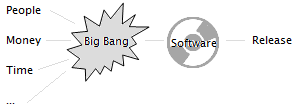
\includegraphics[width=8cm,keepaspectratio=true]{obrazky/big_bang_model.png}
\caption{Model veľkého tresku~\cite{models}}
\label{big_bang_model_fig}
\end{figure}

\section{Model `\textit{programuj a opravuj}'}
\label{code_fix_model}
O~modeli `\textit{programuj a opravuj}'~\ref{code_fix_model_fig} môžeme povedať, že sa z~veľkej časti podobá na model veľkého tresku~\ref{big_bang_model}, no je iteratívny a uznáva potrebu testovania.
Formálny návrh stále nemá veľkú váhu, takže programátori naprogramujú softvér, ten sa otestuje a vráti vývojárom.
Tento postup sa opakuje až kým nie je závažnosť chýb na prijateľnej úrovni.
Tento model sa často objavuje v~iných modeloch ako fáza vývoja softvéru~\cite{Patton}.
\begin{figure}[h]
\centering
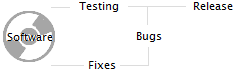
\includegraphics[width=8cm,keepaspectratio=true]{obrazky/code_fix_model.png}
\caption{Model `\textit{programuj a opravuj}'~\cite{models}}
\label{code_fix_model_fig}
\end{figure}

\section{Vodopádový model}
\label{waterfall_model}
Prvý formálne popísaný a asi najznámejší model životného cyklu softvéru~\ref{waterfall_model_fig}.
Bol prezentovaný už v~roku 1970 a vyjadruje postupnosť fáz: získavanie požiadavok, systémová analýza, programovanie, testovanie, implementácia a údržba systému.
Často používaný prí výučbe, je jednoduchý a ľahko sa vysvetľuje.
Definuje a plánuje fázy, čím pomáha dodržovať termíny a výstupy jednotlivých fáz, ale je veľmi málo flexiblný, keďže počíta stým, že požiadavky sa nebudú meniť, takže plánovanie všetkých úloh projektu je treba naplánovať do posledného detaily, čo je náročné a drahé~\cite{Patton}.
\begin{figure}[h]
\centering
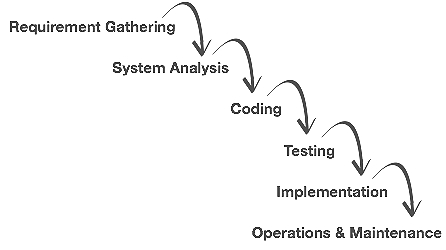
\includegraphics[width=8cm,keepaspectratio=true]{obrazky/waterfall_model.png}
\caption{Vodopádový model~\cite{models}}
\label{waterfall_model_fig}
\end{figure}

\section{V~model}
\label{v_model}
Podobný vodopádovému modelu~\ref{waterfall_model}, no každá fáza pred programovaním má k~sebe doplnkovú fázu, ktorá overuje výsledky fázy pred programovaním~\ref{v_model_fig}.
Napríklad keď sú stanovené požiadavky na softvér, tak hneď môžu byť napísané akceptačné testy~\ref{acceptance_tests}.
No reálne overenie môže nastať až keď je softvér implementovaný.
Vtomto modely je použitých niekoľko testovacích techník, pričom každá z~nich overuje inú časť návrhu, designu, alebo implementácie~\cite{Patton}.
\begin{figure}[h]
\centering
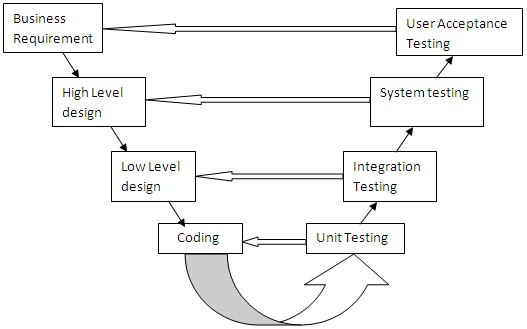
\includegraphics[width=8cm,keepaspectratio=true]{obrazky/v_model.png}
\caption{V~model~\cite{models}}
\label{v_model_fig}
\end{figure}

\section{Špirálový model}
\label{spiral_model}
Vychádza z~vodopádového modelu~\ref{waterfall_model}, no vylepšuje jeho najväčší nedostatok, flexibilu, zavedením iterácii~\ref{spiral_model_fig}.
Každá iterácia má stále súbor výstupov, ktoré musia byť dodržané, no požiadavky sa môžu počas životného cyklu softvéru meniť, čo je v~reáli typické.
Špirálový model je základom filozofie Agilných metodológii.
\begin{figure}[h]
\centering
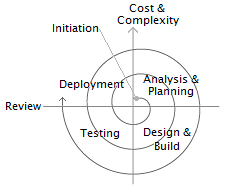
\includegraphics[width=8cm,keepaspectratio=true]{obrazky/spiral_model.png}
\caption{Špirálový model~\cite{models}}
\label{spiral_model_fig}
\end{figure}

\section{Agilné metodológie}
\label{agile}
Agilné metodológie sú modely životného cyklu softvéru postavené na filozofii iteratívnenho a inkrementálneho vývoja softvéru, kde sa požiadavky aj riešenia menia počas vývoja~\ref{agile_pyramide}.
Pojem `\textit{agile}' bol spopularizovaný v~kontexte `\textit{Manifesto for Agile Software Development}'~\cite{agile_manifesto}.
Medzi agilné metodológie patrí aj programovanie riadené testami (\textit{Test driven development}), kde sa testy píšu až pre implementáciou a samotná implementácia je riadená testami. Tento model ďalším dôkazom dôležitosti testovania pri vývoji softvéru.

\begin{figure}[h]
\centering
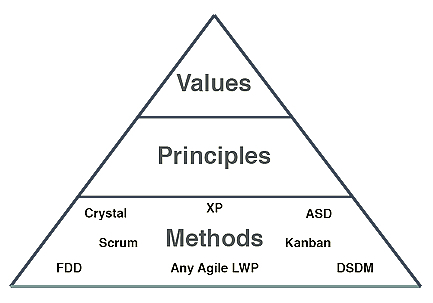
\includegraphics[width=8cm,keepaspectratio=true]{obrazky/agile_pyramide.png}
\caption{Pyramída agilných metodológii~\cite{models}}
\label{agile_pyramide}
\end{figure}

\chapter{Testovanie softvéru}
\label{testing}
Testovanie softvéru je aktivita, ktorá pomáha vyhodnocovať, či chovanie systému zodpovedá tomu, čo je pre neho definované.
Proces testovania pomáha tvorcom softvéru vyhodnotiť, ktoré časti sa správajú správne a ktoré nie, čiže identifikuje chyby v~programe.
Chyby môžu vznikať z~rôznych príčin, no všeobecne platí, že čím skôr sa chyba odhalí, tým ľahšie a teda aj lacnejšie je opraviteľná.
Testovanie je súčasťou verifikácie systému, ktorá je zase súčasťou procesu zabezpečovania kvality softvéru (Quality Assurance, QA).~\cite{hornicky}

\section{Verifikácia a validácia}
Tieto 2 pojmy sú často zamieňané, alebo považované za synonymá.
Aj keď obidva pojmy slúžia na zvyšovanie kvality softvéru, každý z~nich znamená niečo iné.
Verifikácia overuje, či softvér spĺňa technickú špecifikáciu, čiže úlohu na ktorú bol navrhnutý.
Verifikovať sa dá viacerými postupmi:
\begin{itemize}
	\item \textbf{Statická analýza} skúma vlastnosti softvéru bez jeho spúšťania.
	\item \textbf{Dynamická analýza} overuje vlastnosti softvéru práve jeho spúšťaním.
	\item \textbf{Formálna verifikácia} pomocou formálnych metôd overuje, že systém odpovedá špecifikácii.
	\item \textbf{Testovanie} skúma softvér spúšťaním programu za účelom zvýšenia jeho kvality.
\end{itemize}

Validácia potvrdzuje, že softvér spĺňa obchodné podmienky a požiadavky používateľa, nie technickú špecifikáciu.

\section{Metódy testovania softvéru}
Pri návrhu testov je veľmi dôležité do akej miery tester pozná vnútornú štruktúru systému.
Ak sa podieľal na vývoji a dobre ho pozná bude testy navrhovať úplne iným spôsobom ako osoba, ktorá môže mať skúsenosti s~testovaním, no systém nepozná.
Táto kapitola ďalej rozoberá rozdiely v~testovaní pri rozdielnych znalostiach o~systéme.

\subsection{Testovanie čiernej skrinky vs. testovanie bielej skrinky}
\label{blackbox_vs_whitebox}
Pri testovaní metódou čiernej skrinky sa softvér považuje za nepriehľadnú skrinku a tester nemá žiadne informácie o~jej vnútornej štruktúre.
Má informácie o~úlohe softvéru, ale nie o~spôsobe vkonávania tejto úlohy.
Pri tejto metóde je dôležité poznať vlastnosti množiny vstupných dát a vybrať z~nich podmnožinu, ktorá otestuje čo najväčšiu časť možných prípadov.
Tento prístup je výhodný pri odhǎlovaní chýb v~špecifikácii.
Metóda sa používa pri akceptačnom aj regresnom testovaní.

Testovanie bielej skrinky je naopak postavené na fakte, že tester pozná vnútornú štruktúru softvéru.
K~takémuto testovanie je potrebný zdrojový kód, alebo pseudokód popisujúci chovanie softvéru.
Tým, že tester presne pozná štruktúru softvéru dokáže lepšie odhadnúť chovanie systému a pri výbere testovacích prípadov môže voliť napríklad také testovacie prípady aby boli pri testovaní použité všetky vetvy kódu.

Existuje prístup kombinujúci testovanie čiernej a testovanie bielej skrinky, \textbf{testovanie šedej skrinky}.
Tester pozná vnútorné dátové šktruktúry a algoritmy, ale nepozná reálnu imlplementáciu, čiže nedokáže navrhovať testy s~ohľadom na pokrytie kódu.
Tento prístup je čím ďalej, tým viac používaný hlavne kvôli zjednodušeniu návrhu testov bez nutnosti sa podrobne vyznať v~implementácii.

\section{Úrovne testovania softvéru}
\label{testing_levels}
Ako ukazujú modely životného cyklu softvéru, rôzne časti (úrovne) systému je možné testovať pri rôznych príležitostiach. 
Nedá sa testovať stále a všetko, je potrebné určiť kedy budú ktoré časti testované.

\subsection{Jednotkové testy}
\label{unit_tests}
Jednotkové testy (Unit tests) pracujú iba s~jednou jednotkou(komponentom, modulom), ktorú testujú.
Preto sa im niekedy hovorí aj testovanie komponent (Component testing), alebo testovanie modulov (Module testing).
Jednotka by mala byť čo najmenšia, ale dostatočne veľká, aby bola samostatne testovateľná.
Tieto testy sú často robené priamo programátormi a chyby sú odstraňované ihneď ako je to možné.

\subsection{Integračné testy}
\label{integration_tests}
Integračné testy overujú funkčnosť rozhrania medzi komponentami, ktoré môžu byť malé ako pri jednotkových testoch a postupne s~vývojom softvéru sa zväčšovať až sa testuje integrácia celého podsystému do už používaného systému.
Tento prístup sa nazýva inkrementálne integrovanie a chyby dokáže odhaliť pomerne skoro, no je drahý, keďže sa musia simulovať rozhrania, ktoré ešte neboli implementované.
Opačný prístup k~integračný testom sa nazýva integrácia veľkým treskom a testuje sa až keď sú všetky súčasti systému implementované.
Tento prístup je rýchly a jednoduchý, no je náročne zistiť príčinu zlyhania takejto neskorej integrácie.
Ideálny prístup je niekde medzi týmito dvoma extrémnimy prípadmi.
Testovať väčšie súčasti, ktoré by mohli spôsobovať problémy.

\subsection{Systémové testy}
\label{system_tests}
Systémové testy sú robené na takmer hotovom sofvéry a je u~nich vyžadovaná nezávislosť, takže ich robia viaceré tými alebo tretia strana.
Cieľom systémových testov je overiť, že softvér spĺňa špecifikáciu.

\subsection{Akceptačné testy}
\label{acceptance_tests}
Akceptačné testy sú narozdiel od ostatných typov testov zodpovednosťou zákazníka, keďže overujú, či softvér spĺňa požiadavky zákazníka a či je pripravený na prevádzku.
Hľadanie chýb nie je primárnou úlohou akceptačných testov.

\subsection{Regresné testovanie}
\label{regression_tests}
Regresné testy sú robené stále, ak sa zmení nejaká časť softvéru na zaistenie, že nová verzia zdieľa vlastnosti starej a že sa do systému nezaniesli nové chyby.
Toto testovanie prebieha často, takže regresné testy sú veľakrát automatizované.

\section{Automatizácia testov}
\label{tests_automatization}
Testovanie je časovo a finančne náročná činnosť, preto je dobré ho čo najviac automatizovať.
Napríklad ak by sa mal manuálne testovať celý systém po každom vydaní novej verzie, ktorá len opravuje chyby starších verzií, bola by to sizyfovská práca.
No nie všetko testovanie sa dá automatizovať, čo môže byť aj dobre.
Ak automatické testy minú chybu pri prvom spustení, tak tú chybu budú míňať pri každom ďalšom testovaní.
Chyba sa stane imúnna voči testom.

\chapter{Systém Fitcrack} 
\label{Fitcrack}
\textbf{Fitcrack}~\cite{TR_TARZAN} je distribuovaný systém pre obnovu hesiel šifrovaných médii a prelomenie kryptografických hešov.
Pre samotné lámanie hešov používa Hashcat, ktorý je momentálne najrýchlejšie riešenie na trhu.
Správu hosťov a rozdeľovanie úloh zabezpečuje Berkeley Open Infrastructure framework.
Viac o~týchto nástrojoch obsahuje nasledujúca kapitola.
Vlastné súčasti systému Fitcrack sú ďalej popísané v~\ref{Fitcrack_casti}

\section{Nástroje používané systémom Fitcrack}
Táto kapitola popisuje nástroje poživané systémom Fitcrack.
Ich presné fungovanie je pre testovanie nepodstatné vedieť, ale dôležitá je ich funkcia v~systéme.

\subsection{BOINC}
\label{boinc}
\textit{Berkeley Open Infrastructure for Network Computing} (BOINC)~\cite{boincintro} je platforma pre distribuované výpočty, ktorá natívne podporuje dynamické pripojovanie uzlov cez internet.
BOINC bol primárne vytvorený ako nástroj na verejné zdieľanie výpočtových  prostriedkov v~oblastiach ako je meteorológia, medicína, astrofyzika a ďalšie.
Dobrovoľník môže poskytnúť svoje výpočtové kapacity niektorému z~projektov.
Každý projekt sa zaoberá niečím iným, napríklad projekt \textit{Search for Extraterrestrial Intelligence} (SETI)~\cite{SETI} využíva výpočtový výkon dobrovoľníckych staníc na analyzovanie signálov z~vesmíru a hľadanie mimozemského života.
Tento princíp sa nazýva volunteer computing.
BOINC podporuje aj tzv. grid computing, teda zapojenie množstva počítačov a výpočtových stredísk z~rôznych geografických lokalít.

Boinc funguje na princípe server/klient, kde server predstavuje server projektu ku ktorému sa pripája ľubovoľný počet klientov.
Klient sa môže pripojiť z~rôznych zariadení, na ktorom beží rôzny operačný systém a sú vybavené rôznymi jednotkami, na ktorých ma byť prevádzaný výpočet (CPU, GPU, FPGA).
Server zodpovedá za prideľovanie pracovných úloh klientom, zaisťuje sťahovanie najnovších spustiteľných súborov na klientské zariadenia.
Klient môže byť pripojený na viac projektov a sám si určuje koľko výpočtového výkonu chce poskytnúť na jednotlivé úlohy.
BOINC ráta s~prípadmi, kedy sa klienti pripoja alebo odpoja počas výpočtu a ponúka niekoľko spôsobov riešenia, no konkrétne riešenie je implementované tvorcom projektu.
Keďže je BOINC priamo navrhnutý pre distribuovaný výpočet cez internet ponúka množstvo bezpečnostných mechanizmov na prácu v~nedôveryhodnom prostredí.

\subsection{Hashcat}
\label{hashcat}
\textbf{Hashcat}~\cite{hashcatnet} je svetovo najrýchlejším riešením na lámanie hesiel na jednom stroji.
Je zadarmo, má otvorený zdrojový kód, je spustiteľný na Windowse, Linuxe aj na macOS.
Používa OpenCL, ktoré je už dnes kompatibilné s~väčšinou zariadení ( CPU, GPU, DSP, FPGA, … ) a podporuje množstvo formátov.

\textbf{OpenCL} (Open Computing Language)~\cite{opencl} je štandard pre paralelné programovanie na rôznych typov procesorov používaných v~osobných počítačoch, serveroch, mobilných telefónov a vstavaných systémov.


\section{Vlastné časti systému Fitcrack}
\label{Fitcrack_casti}
Ostatné súčasti sú popísané v~tejto kapitole.
\begin{figure}[h]
\centering
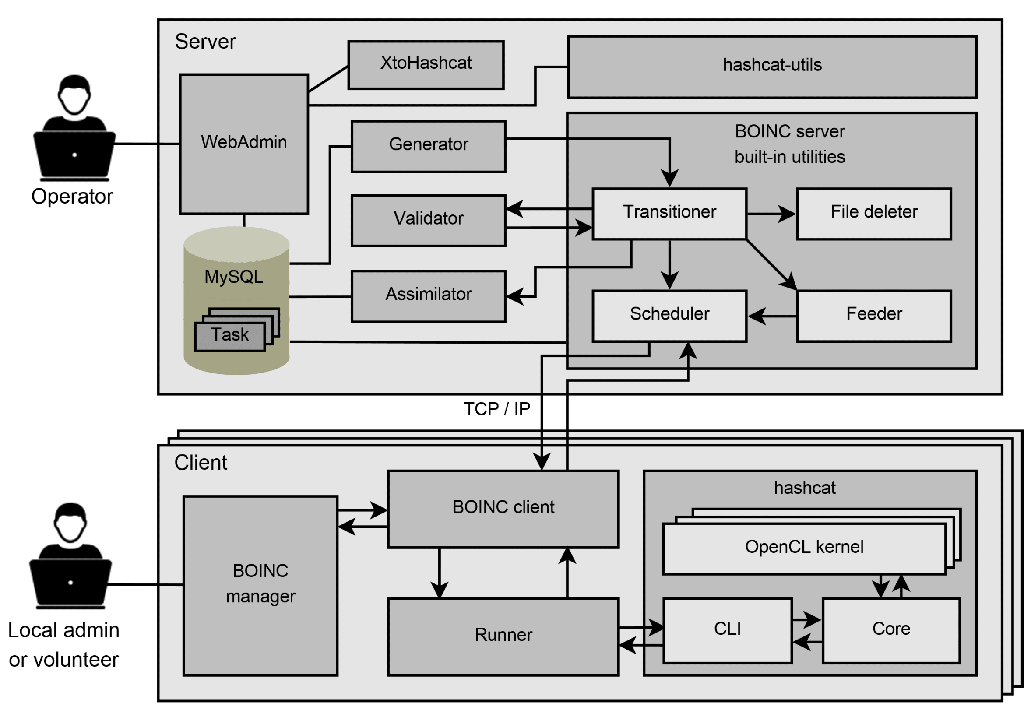
\includegraphics[width=15cm]{obrazky/fc_arch-1.png}
\caption{Architektúra systému Fitcrack.~\cite{TR_TARZAN}}
\label{fig:fc_arch}
\end{figure}

BOINC server, BOINC client, BOINC manager a Validator sú súčasti BOINC-u a neboli nijak modifikované.

Je potrebné testovať iba časti systému aspoň čiastočne implementované tvorcami Fitcracku:
\begin{itemize}
	\label{tests_moduls}
	\item \textbf{Generátor},
	\item \textbf{Asimilátor},
	\item \textbf{Runner},
	\item \textbf{XtoHashcat}.
\end{itemize}

\subsection{WebAdmin}
\label{webadmin}
\textbf{WebAdmin} je grafické užívateľské rozhranie pre ovládanie systému Fitcrack a komunikuje s~databázou pomocou REST API, na ktoré sa zameriava študent Matúš Múčka v~svojej budúcej bakalárskej práci.
Testovanie WebAdmina nie je súčasťou tejto práce, keďže práve prebieha vývoj nového grafického užívateľského rozhrania.

\subsection{REST API}
\label{API}
Vyššie spomenuté \textbf{REST API} slúži na komunikáciu GUI a serverových modulov, konkrétne XtoHashcat a Hashcat-utils, čo sú programy podporujúce Hashcat (overovanie formátu hashu, …).
So zbytkom serverových modulov komunikuje cez databázu.
Toto API je schopné vytvárať nové úlohy, sledovať pripojených klientov, mapovať ich na existujúce úlohy, riadiť výpočet úloh, …

\subsection{XtoHashcat}
\label{xtohashcat}
\textbf{XtoHashcat} je skript v~jazyku Python3 vyvinutý tvorcami systému Fitcrack, ktorý dokáže zobrať na vstup ľubovoľný súbor z~množiny podporovaných súborov a na výstup dá heš pre Hashcat.
To znamená, že dokáže detekovať formát súboru a extrahovať heš zo súboru.

\subsection{Generátor}
\label{generator}
\textbf{Generátor}, alebo Work Generator je BOINC server démon bežiaci v~nekonečnom cykle, v~ktorom generuje nové pracovné úlohy(work units) pre pripojených klientov k~danej úlohe(job).
Generátor vytvára 2 typy úloh: benchmark a normálna.
Benchmark úlohy sa generujú klientom, ktorý sa práve pripojili, alebo keď na danom klientovi nastala chyba.
Normálne úlohy sú pracovné úlohy obsahujúce všetky potrebné informácie pre spustenie klientskej časti systému Fitcrack.
Úloha môže byť v~jednom z~nasledujúcich stavov:
\begin{itemize}
	\item \textbf{0 - ready}. Výpočet neprebieha.
	\item \textbf{1 - finished}. Výpočet bol dokončený a heslo nájdené.
	\item \textbf{2 - exhausted}. Výpočet bol dokončený, ale heslo nebolo nájdené.
	\item \textbf{3 - malformed}. Úloha obsahuje chybný vstup.
	\item \textbf{4 - timeout}. Úloha bola ukončená z~dôvodu prekročenia časového limitu.
	\item \textbf{10 - running}. Prebieha výpočet.
	\item \textbf{12 - finishing}. Negenerujú sa nové pracovné úlohy, ale výpočet stále prebieha na niektorých klientských staniciach.
\end{itemize}
V~module Generátor je implementovaný plánovací algoritmus, ktorý vytvára pracovné úlohy na mieru konkrétnej klientskej stanici.
Princíp činnosti modulu Generátor je popísaný algoritmom~\ref{generator_alg}.

\begin{algorithm}[p]
	\label{generator_alg}
	\caption{Princíp činnosti systemového modulu Generátor}
	\DontPrintSemicolon
	\While{1}{
		\tcc{Inicializácia}
		Zmaž uzly, ktoré sa podieľajú na riešení úlohy, ktorých pracovný balíček
		je už dokončený, buď úspešne (finished) alebo neúspešne
		(exhausted)\;
		Keď niektorý z~balíčkov presiahol stanovenú dobu ukončenia, nastav 
		jeho stav na finished (12)\;
		\ForEach{Bežiaci pracovný balíček (stav $\geq 10$)}{
			\If{Nie je nastavený čas zahájenia}{
				Nastáva čas zahájenia na aktuálny čas\;
			}
			\If{K~balíčku sa viažu masky hesiel}{
				Ulož ích do príslušného poľa, ktoré odpovedá balíčku\;
			}
			Nájdi uzly, ktoré sa majú podieľať na výpočte (a zatiaľ 
			sa nepodieľajú) a ulož ich do databázy\;
			\tcc{Benchmark}
			\ForEach{Pridelený aktívny uzol, ktorý ma stav Benchmark (0)}{
				\If{Uzol ešte nemá naplánovaný benchmark}{
					Naplánuj benchmark pre tento uzol\;
				}
			}
			\tcc{Výpočet}
			\ForEach{Aktívny uzol v~stave Normal (1)}{
				\If{Počet naplánovaných úloh pre uzol $\geq 2$}{
					Pokračuj na ďalší uzol\;
				}
				\If{Stav uzlu je Running (10)}{
					Vygeneruj novú úlohu podľa typu balíčka, prípadne
					znovu prideľ nedokončené úlohy\;
				}
				\If{Stav uzle je Finished (12)}{
					Znovu prideľ nedokončené úlohy, ak taká neexistuje,
					nastav stav uzlu na Done (3)\;
				}
				\tcc{Kontrola stavu}
				\If{Stav balíčka je Finished (12) a neobsahuje žiadne úlohy}{
					\eIf{Aktuálny čas > plánovaný Čas ukončenia}{
						Nastav stav balíčka na Timeout (4)\;
					}{
						\eIf{Aktuálny index $\geq$ maximálny index}{
							Nastav stav balíčku na Exhausted (2)\;
							\tcc{vyčerpaný stavový priestor}
						}{
							Nastav stav balíčku na Ready(0)\;
							\tcc{výpočet bol pozastavený}
						}
					}
				}
			}
		}
		Čakaj stanovený časový interval\;
	}
\end{algorithm}

\subsection{Asimilátor}
\label{asimilator}
\textbf{Asimilátor} je takisto BOINC server démon, ktorý spracováva valídne výsledky.
Nekonečný cyklus v~ktorom beží je poskytnutý BOINC-om, ale samotná akcia, ktorá sa vykonáva pri prijatí výsledku je implementovaná tvorcami Fitcrack-u.
Funkčnosť akcie je prezentovaná algoritmom~\ref{asimilator_alg}.

\begin{algorithm}[h]
	\label{asimilator_alg}
	\caption{Princíp činnosti modulu Asimilátor}
	\DontPrintSemicolon
	\While{1}{
		\Switch{typ}{
			\Case{benchmark}{
				\eIf{Výsledok je v~poriadku (kód 0)}{
					Prečítaj zmeraný výkon a ulož ho do databázy\;
				}{
					Naplánuj nový benchmark na dlhší čas\;
				}
			}\Case{normal}{
				\eIf{Heslo bol nájdené (kód 0)}{
					Prečítaj heslo a ulož ho do databázy (prípadne aj do cache)\;
					Uprav stav úlohy na Finished (1)\;
					Pošli všetkým zapojeným uzlom pokyn k~ukončeniu výpočtu\;
					Odstráň/archivuj nedokončené úlohy\;
					Prečítaj časvýpočtu úlohy a ulož ho\;
				}{
					\eIf{Heslo nebolo nájdené (kód 1)}{
						Aktualizuj veľkosť úlohy\;
						Aktualizuj počet overených hesiel\;
					}{
						\tcc{Chyba výpočtu}
						Zruš úlohy pro daný uzol a nastav im príznak retry\;
						Vynuluj výkon uzu v~databázi a naplánuj nový benchmark\;
					}
				}
			}
		}
	}
\end{algorithm}

\subsection{Runner}
\label{runner}
\textbf{Runner} je aplikácia bežiaca na klientskom počítači ovládajúca Hashcat.
BOINC server pošle údaje o~pracovnej úlohe BOINC klientovi, ktorý pomocou systémových volaní spúšťa runner a predáva mu tieto informácie v~podobe vstupných súborov.
Runner následne tieto informácie predá nástroju Hashcat.
Runner sleduje stav výpočtu a po je jeho skončení predá výsledky BOINC klientovi.


Generátor a Asimilátor komunikujú výhradne pomocou databázy, kde to validátor a runner riadi priamo BOINC.
Okrem BOINC klienta nie je potrebné na klientskom zariadení nič inštalovať, BOINC klient sám zo servera sťahuje najnovšie spustiteľné súbory v~závislosti na architektúra klientského zariadenia.

\chapter{Návrh testov pre systém Fitcrack}
K~návrhu testov pre systém Fitcrack potrebujeme poznať architektúru systému Fitcrack~\ref{Fitcrack} a moduly, ktoré budú testované~\ref{tests_moduls}.
Nápovedu kedy sa budú jednotlivé moduly testovať by nám mala poskytnúť kapitola~\ref{tests_design} a spôsoby testovania popisuje zase kapitola~\ref{testing_levels}. 
 Požiadavky na testy vyplývajú z~úvodu práce, ako aj z~kapitoly o~systéme Fitcrack~\ref{Fitcrack}.
 Táto časť práce používa znalosti z~predošlých kapitol a jej súčasťou je návrh testov pre systém Fitcrack, ktorý je podložený znalosťami z~kapitol~\ref{tests_design}, \ref{testing} a \ref{Fitcrack}.

 Ideálne by sa návrh testov mal držať V~modelu životného cyklu softvéru~\ref{v_model}, no keďže systém Fitcrack je vyvíjaný pre väčšie organizácie, ktoré si určujú vlastnosti systému a tie sa neustále menia, tak vývoj systému, ako aj jeho testov musí prebiehať iteratívne, tak ako to popisuje špirálový model~\ref{spiral_model}

Pre testovanie systému Fitcrack som sa rozhodol použiť kombináciu jednotkových (unit) testov a integračného testovania.
Jednotkové testy nedokážu odhaliť chyby na serveri spojené s~komunikáciou cez databázu a integračné testy sú v~systéme Fitcrack možné iba cez databázu, čo je jediné rozhranie, ktoré väčšina modulov používa a tieto testy nemajú dostatočné pokrytie funkcionality systému.
Kombinácia týchto testov bude takisto slúžiť na regresné testovanie.
Z~pohľadu metódy testovania sa na moduly budem pozerať ako na šedé skrinky~\ref{blackbox_vs_whitebox}, keďže poznám ako moduly fungujú, no presnú implementáciu nepoznám.
Testovanie bude prebiehať v~reálnom prostredí a úplne overenie funkčnosti systému sa prevedie až keď sa k~projektu pripojí klient.

\section{Integračné testy}
\textbf{Integračné testy}~\ref{integration_tests} budú implementované v~jazyku Python3 a bude použitý framework unittest.
Unittest, tiež známy ako PyUnit,~\cite{unittest} je štandardný unit test framework pre Python.
Pre implementáciu integračných testov som si vybral Python hlavne kvôli jeho jednoduchosti, použiteľnosti frameworku unittest, možnosti jednoducho používať REST API, ako aj pripojenie do databázy.
Testovací prípad (test case) bude pozostávať z~viacerých častí, keďže na začiatku je potrebné overiť, či je testovaný endpoint REST API dostupný, či nám vráti očakávanú hodnotu a nakoniec aj či zmena v~databázi odpovedá vrátenej hodnote.
Na zmenu v~databázi by mal reagovať niektrorý z~testovaných serverových modulov a vykonať akciu, ktorú je potrebné skontrolovať.
Jeden testovací prípad popisuje algoritmus~\ref{integration_test_alg}.

\begin{algorithm}[h]
	\label{integration_test_alg}
	\caption{Princíp integračných testov.}
	\DontPrintSemicolon
	Zavolaj endpoint REST API~\ref{API}\;
	Skontroluje hodnotu, ktorú vrátilo API s~referenčnou hodnotou\;
	\If{Akcia vykoná zmenu v~databázi}{
		Skontroluj, či databáza obsahuje správny záznam\;
		\tcc{Zmenu v~databázi je možné porovnať ako s~vráteným výsledkom, tak aj s~referenčnou hodnotou.}
		}
	Počkaj, kým testovaný serverový modul vykoná akciu\;
	Skontroluj správnosť vykonanej akcie\;
\end{algorithm}

\section{Jednotkové testy}
\textbf{Jednotkové testy}~\ref{unit_tests} budú napísané pre Generátor, Asimilátor a Runner.
Všetky tieto moduly sú napísané v~C/C++, takže je možné použiť napríklad Google Test framework.
Moduly budú testované metódou šedej skrinky~\ref{blackbox_vs_whitebox}, keďže ich implementácia je pomerne zložitá, no je potrebné pokryť čo najväčšiu časť kódu, hlavne pri module Generátor~\ref{generator} a klientskej časti, module Runner~\ref{runner}.

Keďže je Generátor asi najzložitejší modul a jeho plánovací algoritmus sa integračným testovaním overiť nedá, je potrebné implementovať jednotkové testy pre všetky časti tohto modulu samostatne.
Je potrebné testovať nasledujúce funkcie:
\begin{itemize}
	\item plánovanie pracovnej úlohy typu benchmark,
	\item plánovanie normálne pracovnej úlohy,
	\item plánovací algoritmus (čierna skrinka),
	\item prerozdeľovanie nedokončených pracovných úloh,
	\item ukončenie výpočtu na ostatných staniciach po nájdení hesla.
\end{itemize}

Princíp činnosti modulu Asimilátor~\ref{asimilator} je pomerne jednoduchý, ale takisto jeho správnosť sa integračným testovaním overiť nedá.
Celý modul Asimilátor bude braný ako jedna šedá skrinka a podľa toho budú napísané testy.

Runner bude testovaný pred spustením benchmarku na klientovi, z~nasledujúcich dôvodov:
\begin{itemize}
\item Kedže runner musí pracovať rovnako na rôznych platformách, musí byť aj testovaný na rôznych platformách
\item Runner priamo spúšťa a kontroluje Hashcat, ktorého správanie závisí od zariadenia na ktorom je spustený (ovládače, typ GPU, typ CPU, …)
\item Benchmark sa spúšťa pre každého klienta keď sa 1.
krát pripojí, alebo sa niečo zmenilo, alebo nastala chyba
\item Pri benchmarku je spúšťaný runner a Hashcat
\item Simulovanie chýb Hashcatu by bolo veľmi náročné a neefektívne 
\end{itemize}
Pri module Runner bude testované:
\begin{itemize}
	\item komunikácia so serverom,
	\item schopnosť správne čítať konfiguračný súbor,
	\item spustenie akcie benchmark,
	\item správnosť kombinácie argumentov pri spúšťaní aplikácie Hashcat~\ref{hashcat},
	\item ďalšie funkcie pridávané počas vývoja.
\end{itemize}

\chapter{Záver}
V~rámci práce boli zhromaždené a naštudované informáciu potrebné pre návrh a implementáciu testov, pričom návrh testov je súčasťou tejto práce.
Potrebné informácie sú rozdelené na: požiadavky na testy systému, prehľad modelov životného cyklu vývoja softvéru, teórie testovania, princíp systému Fitcrack a návrhu samotných testov.
Takisto bola overená funkčnosť architektúry akceptačných testov pomocou skriptu, ktorý dokáže čítať a interpretovať údaje z~databázy.
Problém by mohol byť s~posielaním výsledkov testovania runner-u na klientovi, no spolieham sa na BOINC a funkcionalitu.

Ďalšia práca by sa mala zamerať na meranie pokrytia kódu/logiky systému testovacími prípadmi a samotnú iplementáciu testovacích prípadov, pre oba spôsoby testovania.
Je potrebné stanoviť metriky a spôsoby merania pokrytia logiky systému testovacími prípadmi.
Pre implementáciu jednotkových testov je vítaná úzka spolupráca s~vývojármi konkrétnych modulov, no nie je vyžadovaná.
Kapitola o~testovaní softvéru~\ref{testing} obsahuje veľké množstvo pojmov, ktoré nie sú formálne definované, preto by bolo vhodné ešte pred samotnou implementáciou testov naštudovať a doplniť tieto definície.

Testy systému by mohli byť použité aj na diagnostiku softvéru v~prevádzke, no to bude vyžadovať spoluprácu s~vývojármi WebAdmin-a a REST API, ktoré komunikuje so serverovými modulmi, aby výsledky testov/ diagnostiky mohli byť vizualizované užívateľovi.
%=========================================================================

  \subfile{kapitoly/xchrip00_sep-01-uvod.tex}
  \subfile{kapitoly/xchrip00_sep-02-testovanie.tex}
  \subfile{kapitoly/xchrip00_sep-03-poziadavky.tex}
  \subfile{kapitoly/xchrip00_sep-04-fitcrack.tex}
  \subfile{kapitoly/xchrip00_sep-05-navrh.tex}
  \subfile{kapitoly/xchrip00_sep-06-implementacia.tex}
  \subfile{kapitoly/xchrip00_sep-07-zaver.tex}
  
  % Kompilace po částech (viz výše, nutno odkomentovat)
  % Compilation piecewise (see above, it is necessary to uncomment it)
  %\subfile{projekt-01-uvod-introduction}
  % ...
  %\subfile{chapters/projekt-05-conclusion}


  % Pouzita literatura / Bibliography
  % ----------------------------------------------
\ifslovak
  \makeatletter
  \def\@openbib@code{\addcontentsline{toc}{chapter}{Literatúra}}
  \makeatother
  \bibliographystyle{bib-styles/czechiso}
\else
  \ifczech
    \makeatletter
    \def\@openbib@code{\addcontentsline{toc}{chapter}{Literatura}}
    \makeatother
    \bibliographystyle{bib-styles/czechiso}
  \else 
    \makeatletter
    \def\@openbib@code{\addcontentsline{toc}{chapter}{Bibliography}}
    \makeatother
    \bibliographystyle{bib-styles/englishiso}
  %  \bibliographystyle{alpha}
  \fi
\fi
  \begin{flushleft}
  \bibliography{xchrip00_sep-20-literatura-bibliography}
  \end{flushleft}

  % vynechani stranky v oboustrannem rezimu
  % Skip the page in the two-sided mode
  \iftwoside
    \cleardoublepage
  \fi

  % Prilohy / Appendices
  % ---------------------------------------------
  \appendix
\ifczech
  \renewcommand{\appendixpagename}{Přílohy}
  \renewcommand{\appendixtocname}{Přílohy}
  \renewcommand{\appendixname}{Příloha}
\fi
\ifslovak
  \renewcommand{\appendixpagename}{Prílohy}
  \renewcommand{\appendixtocname}{Prílohy}
  \renewcommand{\appendixname}{Príloha}
\fi
%  \appendixpage

% vynechani stranky v oboustrannem rezimu
% Skip the page in the two-sided mode
%\iftwoside
%  \cleardoublepage
%\fi
  
\ifslovak
%  \section*{Zoznam príloh}
%  \addcontentsline{toc}{section}{Zoznam príloh}
\else
  \ifczech
%    \section*{Seznam příloh}
%    \addcontentsline{toc}{section}{Seznam příloh}
  \else
%    \section*{List of Appendices}
%    \addcontentsline{toc}{section}{List of Appendices}
  \fi
\fi
  \startcontents[chapters]
  \setlength{\parskip}{0pt}
  % seznam příloh / list of appendices
  % \printcontents[chapters]{l}{0}{\setcounter{tocdepth}{2}}
  
  \ifODSAZ
    \setlength{\parskip}{0.5\bigskipamount}
  \else
    \setlength{\parskip}{0pt}
  \fi
  
  % vynechani stranky v oboustrannem rezimu
  \iftwoside
    \cleardoublepage
  \fi
  
  % Přílohy / Appendices
 % % Tento soubor nahraďte vlastním souborem s přílohami (nadpisy níže jsou pouze pro příklad)
% This file should be replaced with your file with an appendices (headings below are examples only)

% Umístění obsahu paměťového média do příloh je vhodné konzultovat s vedoucím
% Placing of table of contents of the memory media here should be consulted with a supervisor
%\chapter{Obsah přiloženého paměťového média}

%\chapter{Manuál}

%\chapter{Konfigurační soubor} % Configuration file

%\chapter{RelaxNG Schéma konfiguračního souboru} % Scheme of RelaxNG configuration file

%\chapter{Plakát} % poster

\chapter{Jak pracovat s~touto šablonou}
\label{jak}

V~této kapitole je uveden popis jednotlivých částí šablony, po kterém následuje stručný návod, jak s~touto šablonou pracovat. 

Jedná se o~přechodnou verzi šablony. Nová verze bude zveřejněna do~konce roku 2017 a~bude navíc obsahovat nové pokyny ke správnému využití šablony, závazné pokyny k~vypracování bakalářských a diplomových prací (rekapitulace pokynů, které jsou dostupné na~webu) a nezávazná doporučení od vybraných vedoucích, která již teď najdete na~webu (viz odkazy v~souboru s~literaturou). Jediné soubory, které se v~nové verzi změní, budou \texttt{projekt-01-kapitoly-chapters.tex} a \texttt{projekt-30-prilohy-appendices.tex}, jejichž obsah každý student vymaže a nahradí vlastním. Šablonu lze tedy bez problémů využít i~v~současné verzi.

\section*{Popis částí šablony}

Po rozbalení šablony naleznete následující soubory a adresáře:
\begin{DESCRIPTION}
  \item [bib-styles] Styly literatury (viz níže). 
  \item [obrazky-figures] Adresář pro Vaše obrázky. Nyní obsahuje placeholder.pdf (tzv. TODO obrázek, který lze použít jako pomůcku při tvorbě technické zprávy), který se s~prací neodevzdává. Název adresáře je vhodné zkrátit, aby byl jen ve zvoleném jazyce.
  \item [template-fig] Obrázky šablony (znak VUT).
  \item [fitthesis.cls] Šablona (definice vzhledu).
  \item [Makefile] Makefile pro překlad, počítání normostran, sbalení apod. (viz níže).
  \item [projekt-01-kapitoly-chapters.tex] Soubor pro Váš text (obsah nahraďte).
  \item [projekt-20-literatura-bibliography.bib] Seznam literatury (viz níže).
  \item [projekt-30-prilohy-appendices.tex] Soubor pro přílohy (obsah nahraďte).
  \item [projekt.tex] Hlavní soubor práce -- definice formálních částí.
\end{DESCRIPTION}

Výchozí styl literatury (czechiso) je od Ing. Martínka, přičemž anglická verze (englishiso) je jeho překladem s~drobnými modifikacemi. Oproti normě jsou v~něm určité odlišnosti, ale na FIT je dlouhodobě akceptován. Alternativně můžete využít styl od Ing. Radima Loskota nebo od Ing. Radka Pyšného\footnote{BP Ing. Radka Pyšného \url{http://www.fit.vutbr.cz/study/DP/BP.php?id=7848}}. Alternativní styly obsahují určitá vylepšení, ale zatím nebyly řádně otestovány větším množstvím uživatelů. Lze je považovat za beta verze pro zájemce, kteří svoji práci chtějí mít dokonalou do detailů a neváhají si nastudovat detaily správného formátování citací, aby si mohli ověřit, že je vysázený výsledek v~pořádku.

Makefile kromě překladu do PDF nabízí i další funkce:
\begin{itemize}
  \item přejmenování souborů (viz níže),
  \item počítání normostran,
  \item spuštění vlny pro doplnění nezlomitelných mezer,
  \item sbalení výsledku pro odeslání vedoucímu ke kontrole (zkontrolujte, zda sbalí všechny Vámi přidané soubory, a případně doplňte).
\end{itemize}

Nezapomeňte, že vlna neřeší všechny nezlomitelné mezery. Vždy je třeba manuální kontrola, zda na konci řádku nezůstalo něco nevhodného -- viz Internetová jazyková příručka\footnote{Internetová jazyková příručka \url{http://prirucka.ujc.cas.cz/?id=880}}.

\paragraph {Pozor na číslování stránek!} Pokud má obsah 2 strany a na 2. jsou jen \uv{Přílohy} a~\uv{Seznam příloh} (ale žádná příloha tam není), z~nějakého důvodu se posune číslování stránek o~1 (obsah \uv{nesedí}). Stejný efekt má, když je na 2. či 3. stránce obsahu jen \uv{Literatura} a~je možné, že tohoto problému lze dosáhnout i jinak. Řešení je několik (od~úpravy obsahu, přes nastavení počítadla až po sofistikovanější metody). \textbf{Před odevzdáním proto vždy překontrolujte číslování stran!}


\section*{Doporučený postup práce se šablonou}

\begin{enumerate}
  \item \textbf{Zkontrolujte, zda máte aktuální verzi šablony.} Máte-li šablonu z~předchozího roku, na stránkách fakulty již může být novější verze šablony s~aktualizovanými informacemi, opravenými chybami apod.
  \item \textbf{Zvolte si jazyk}, ve kterém budete psát svoji technickou zprávu (česky, slovensky nebo anglicky) a svoji volbu konzultujte s~vedoucím práce (nebyla-li dohodnuta předem). Pokud Vámi zvoleným jazykem technické zprávy není čeština, nastavte příslušný parametr šablony v~souboru projekt.tex (např.: \verb|documentclass[english]{fitthesis}| a přeložte prohlášení a poděkování do~angličtiny či slovenštiny.
  \item \textbf{Přejmenujte soubory.} Po rozbalení je v~šabloně soubor \texttt{projekt.tex}. Pokud jej přeložíte, vznikne PDF s~technickou zprávou pojmenované \texttt{projekt.pdf}. Když vedoucímu více studentů pošle \texttt{projekt.pdf} ke kontrole, musí je pracně přejmenovávat. Proto je vždy vhodné tento soubor přejmenovat tak, aby obsahoval Váš login a (případně zkrácené) téma práce. Vyhněte se však použití mezer, diakritiky a speciálních znaků. Vhodný název může být např.: \uv{\texttt{xlogin00-Cisteni-a-extrakce-textu.tex}}. K~přejmenování můžete využít i přiložený Makefile:
\begin{verbatim}
make rename NAME=xlogin00-Cisteni-a-extrakce-textu
\end{verbatim}
  \item Vyplňte požadované položky v~souboru, který byl původně pojmenován \texttt{projekt.tex}, tedy typ, rok (odevzdání), název práce, svoje jméno, ústav (dle zadání), tituly a~jméno vedoucího, abstrakt, klíčová slova a další formální náležitosti.
  \item Nahraďte obsah souborů s~kapitolami práce, literaturou a přílohami obsahem svojí technické zprávy. Jednotlivé přílohy či kapitoly práce může být výhodné uložit do~samostatných souborů -- rozhodnete-li se pro toto řešení, je doporučeno zachovat konvenci pro názvy souborů, přičemž za číslem bude následovat název kapitoly. 
  \item Nepotřebujete-li přílohy, zakomentujte příslušnou část v~\texttt{projekt.tex} a příslušný soubor vyprázdněte či smažte. Nesnažte se prosím vymyslet nějakou neúčelnou přílohu jen proto, aby daný soubor bylo čím naplnit. Vhodnou přílohou může být obsah přiloženého paměťového média.
  \item Nascanované zadání uložte do souboru \texttt{zadani.pdf} a povolte jeho vložení do práce parametrem šablony v~projekt.tex (\verb|documentclass[zadani]{fitthesis}|).
  \item Nechcete-li odkazy tisknout barevně (tedy červený obsah -- bez konzultace s~vedoucím nedoporučuji), budete pro tisk vytvářet druhé PDF s~tím, že nastavíte parametr šablony pro tisk: (\verb|documentclass[zadani,print]{fitthesis}|).  Barevné logo se nesmí tisknout černobíle!
  \item Vzor desek, do kterých bude práce vyvázána, si vygenerujte v~informačním systému fakulty u~zadání. Pro disertační práci lze zapnout parametrem v~šabloně (více naleznete v~souboru fitthesis.cls).
  \item Nezapomeňte, že zdrojové soubory i (obě verze) PDF musíte odevzdat na CD či jiném médiu přiloženém k~technické zprávě.
\end{enumerate}

Obsah práce se generuje standardním příkazem \tt \textbackslash tableofcontents \rm (zahrnut v~šabloně). Přílohy jsou v~něm uvedeny úmyslně.

\subsection*{Pokyny pro oboustranný tisk}
\begin{itemize}
\item \textbf{Oboustranný tisk je doporučeno konzultovat s~vedoucím práce.}
\item Je-li práce tištěna oboustranně a její tloušťka je menší než tloušťka desek, nevypadá to dobře.
\item Zapíná se parametrem šablony: \verb|\documentclass[twoside]{fitthesis}|
\item Po vytištění oboustranného listu zkontrolujte, zda je při prosvícení sazební obrazec na obou stranách na stejné pozici. Méně kvalitní tiskárny s~duplexní jednotkou mají často posun o~1--3 mm. Toto může být u~některých tiskáren řešitelné tak, že vytisknete nejprve liché stránky, pak je dáte do stejného zásobníku a vytisknete sudé.
\item Za titulním listem, obsahem, literaturou, úvodním listem příloh, seznamem příloh a případnými dalšími seznamy je třeba nechat volnou stránku, aby následující část začínala na liché stránce (\textbackslash cleardoublepage).
\item  Konečný výsledek je nutné pečlivě překontrolovat.
\end{itemize}

\subsection*{Styl odstavců}

Odstavce se zarovnávají do bloku a pro jejich formátování existuje více metod. U~papírové literatury je častá metoda s~použitím odstavcové zarážky, kdy se u~jednotlivých odstavců textu odsazuje první řádek odstavce asi o~jeden až dva čtverčíky (vždy o~stejnou, předem zvolenou hodnotu), tedy přibližně o~dvě šířky velkého písmene M základního textu. Poslední řádek předchozího odstavce a~první řádek následujícího odstavce se v~takovém případě neoddělují svislou mezerou. Proklad mezi těmito řádky je stejný jako proklad mezi řádky uvnitř odstavce. \cite{fitWeb} Další metodou je odsazení odstavců, které je časté u~elektronické sazby textů. První řádek odstavce se při této metodě neodsazuje a mezi odstavce se vkládá vertikální mezera o~velikosti 1/2 řádku. Obě metody lze v~kvalifikační práci použít, nicméně často je vhodnější druhá z~uvedených metod. Metody není vhodné kombinovat.

Jeden z~výše uvedených způsobů je v~šabloně nastaven jako výchozí, druhý můžete zvolit parametrem šablony \uv{\tt odsaz\rm }.

\subsection*{Užitečné nástroje}
\label{nastroje}

Následující seznam není výčtem všech využitelných nástrojů. Máte-li vyzkoušený osvědčený nástroj, neváhejte jej využít. Pokud však nevíte, který nástroj si zvolit, můžete zvážit některý z~následujících:

\begin{description}
	\item[\href{http://miktex.org/download}{MikTeX}] \LaTeX{} pro Windows -- distribuce s~jednoduchou instalací a vynikající automatizací stahování balíčků.
	\item[\href{http://texstudio.sourceforge.net/}{TeXstudio}] Přenositelné opensource GUI pro \LaTeX{}.  Ctrl+klik umožňuje přepínat mezi zdrojovým textem a PDF. Má integrovanou kontrolu pravopisu, zvýraznění syntaxe apod. Pro jeho využití je nejprve potřeba nainstalovat MikTeX.
	\item[\href{http://www.winedt.com/}{WinEdt}] Ve Windows je dobrá kombinace WinEdt + MiKTeX. WinEdt je GUI pro Windows, pro jehož využití je nejprve potřeba nainstalovat \href{http://miktex.org/download}{MikTeX} či \href{http://www.tug.org/texlive/}{TeX Live}. 
	\item[\href{http://kile.sourceforge.net/}{Kile}] Editor pro desktopové prostředí KDE (Linux). Umožňuje živé zobrazení náhledu. Pro jeho využití je potřeba mít nainstalovaný \href{http://www.tug.org/texlive/}{TeX Live} a Okular. 
	\item[\href{http://jabref.sourceforge.net/download.php}{JabRef}] Pěkný a jednoduchý program v~Javě pro správu souborů s~bibliografií (literaturou). Není potřeba se nic učit -- poskytuje jednoduché okno a formulář pro editaci položek.
	\item[\href{https://inkscape.org/en/download/}{InkScape}] Přenositelný opensource editor vektorové grafiky (SVG i PDF). Vynikající nástroj pro tvorbu obrázků do odborného textu. Jeho ovládnutí je obtížnější, ale výsledky stojí za to.
	\item[\href{https://git-scm.com/}{GIT}] Vynikající pro týmovou spolupráci na projektech, ale může výrazně pomoci i jednomu autorovi. Umožňuje jednoduché verzování, zálohování a přenášení mezi více počítači.
	\item[\href{http://www.overleaf.com/}{Overleaf}] Online nástroj pro \LaTeX{}. Přímo zobrazuje náhled a umožňuje jednoduchou spolupráci (vedoucí může průběžně sledovat psaní práce), vyhledávání ve zdrojovém textu kliknutím do PDF, kontrolu pravopisu apod. Zdarma jej však lze využít pouze s~určitými omezeními (někomu stačí na disertaci, jiný na ně může narazit i při psaní bakalářské práce) a pro dlouhé texty je pomalejší.
\end{description}

Pozn.: Overleaf nepoužívá Makefile v~šabloně -- aby překlad fungoval, je nutné kliknout pravým tlačítkem na \tt projekt.tex \rm a zvolit \uv{Set as Main File}.


\subsection*{Užitečné balíčky pro \LaTeX}

Studenti při sazbě textu často řeší stejné problémy. Některé z~nich lze vyřešit následujícími balíčky pro \LaTeX:

\begin{itemize}
  \item \verb|amsmath| -- rozšířené možnosti sazby rovnic,
  \item \verb|float, afterpage, placeins| -- úprava umístění obrázků,
  \item \verb|fancyvrb, alltt| -- úpravy vlastností prostředí Verbatim, 
  \item \verb|makecell| -- rozšíření možností tabulek,
  \item \verb|pdflscape, rotating| -- natočení stránky o~90 stupňů (pro obrázek či tabulku),
  \item \verb|hyphenat| -- úpravy dělení slov,
  \item \verb|picture, epic, eepic| -- přímé kreslení obrázků.
\end{itemize}

Některé balíčky jsou využity přímo v~šabloně (v~dolní části souboru fitthesis.cls). Nahlédnutí do jejich dokumentace může být rovněž užitečné.

Sloupec tabulky zarovnaný vlevo s~pevnou šířkou je v~šabloně definovaný \uv{L} (používá se jako \uv{p}).


  
  % Kompilace po částech (viz výše, nutno odkomentovat)
  % Compilation piecewise (see above, it is necessary to uncomment it)
  %\subfile{xchrip00_sep-30-prilohy-appendices}
  
\end{document}
